\documentclass[10pt]{article}

\usepackage[margin=1in]{geometry}
\usepackage[T1]{fontenc}
\usepackage{lmodern}
\usepackage{setspace}
\usepackage{amsmath, amssymb}
\usepackage{tikz}
\usetikzlibrary{shapes}
\usepackage{enumitem}
\usepackage[normalem]{ulem}
\usepackage{float}
\usepackage{xcolor}
\usepackage[hidelinks]{hyperref}
\usepackage{tocloft}



\setlength{\parindent}{0pt}
\setlength{\parskip}{0.35em}

\onehalfspacing

\begin{document}

\begin{titlepage}
\centering

\vspace*{3cm}

{\LARGE MIE Lecture Notes}\\[0.4cm]
{\large Probability and Statistics}\\[2cm]

{\large Contents}

\vspace{1cm}

\noindent
Chapter 1: \dotfill
\hyperref[chap:one]{\pageref*{chap:one}}

\vspace{0.5cm}

\noindent
Chapter 2: 
\dotfill
\hyperref[chap:two]{\pageref*{chap:two}}

\vfill

\end{titlepage}

\newpage


\section*{Chapter 1}
\label{chap:one}


\subsection*{Statistics Definitions}

\textbf{Global definition:} Statistics involves collecting, organizing, summarizing, presenting, and analyzing data, as well as making inferences, conclusions, and decisions based on data.

\textbf{Statistical definition:} A \underline{statistic} is a numerical value calculated from data (e.g.\ mean, proportion, standard deviation).

\vspace{0.5em}

\begin{center}
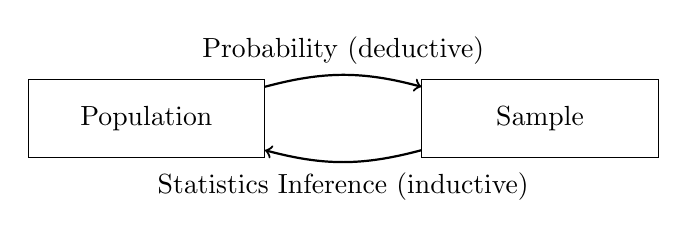
\begin{tikzpicture}[
    box/.style={draw, rectangle, minimum width=3cm, minimum height=1cm},
    arrow/.style={->, thick}
]

\node[box] (pop) at (0,0) {Population};
\node[box] (samp) at (5,0) {Sample};

% top line
\draw[arrow] (pop) to[bend left=15] node[above] {Probability (deductive)} (samp);

% bottom line
\draw[arrow] (samp) to[bend left=15] node[below] {Statistics Inference (inductive)} (pop);

\end{tikzpicture}
\end{center}


\subsection*{Basic Terminology}
\underline{Individuals}: Objects on which data are collected (people, animals, plots of land, etc.).\\
\underline{Variable}: Any characteristic of an individual.\\
\underline{Population}: The entire group of individuals of interest.\\
\underline{Sample}: A subset of individuals taken from the population.\\
\underline{Statistical Inference}: Drawing conclusions about a population based on a sample.


\subsection*{Sampling Methods}

\underline{Simple Random Sample (SRS):}
\begin{itemize}
  \item Every possible group of size $n$ has an equal chance of being selected.
  \item Helps avoid bias in sampling.
  \item Can be selected using random number tables or software.
\end{itemize}

\underline{Stratified Random Sampling:}
\begin{itemize}
  \item The population is divided into \underline{homogeneous groups} 
        \textit{(individuals are similar with respect to the variable being studied)} 
        called \underline{strata}.
  \item A simple random sample is taken from each \underline{stratum}. 
        \textit{(one subgroup of the population created)}
  \item Ensures that important subgroups are neither over nor under represented.
\end{itemize}

\subsection*{Types of Variables}

\underline{Categorical Variable}: Places individuals into categories (e.g.\ gender, major). These are qualitative.

\underline{Quantitative Variable}: Takes numerical values for which arithmetic operations are meaningful.

\begin{itemize}
    \item \underline{Discrete}
    \item \underline{Continuous}
\end{itemize}


\subsection*{Distributions}

\underline{Distribution}: Describes what values a variable takes and how often those values occur.
When examining a distribution, look for:
\begin{itemize}
    \item \textbf{Shape}
    \item \textbf{Center}
    \item \textbf{Spread}
    \item \textbf{Outliers}
\end{itemize}
\underline{Outlier}: An individual value that falls outside the overall pattern of the data.

\subsection*{Describing Distributions with Numbers}

\underline{Central Tendency}: Describes where the data cluster or center.

\underline{Central Tendency}: Describes where the data cluster or center.
\begin{itemize}
    \item \underline{Mean}: average value
    \item \underline{Median}: middle value
\end{itemize}

\bigskip

\noindent
\underline{Mean (Arithmetic Mean):}
\[
\boxed{
\bar{x} = \frac{1}{n}\sum_{i=1}^{n} x_i
}
\]

\bigskip

\noindent
\underline{Median:}
\[
\boxed{
\tilde{x} =
\begin{cases}
x_{\left(\frac{n+1}{2}\right)}, & \text{if } n \text{ is odd} \\[6pt]
\displaystyle \frac{x_{\left(\frac{n}{2}\right)} + x_{\left(\frac{n}{2}+1\right)}}{2}, & \text{if } n \text{ is even}
\end{cases}
}
\]

\bigskip

\textbf{\textcolor{blue}{Theorem 1.1}}
\begin{enumerate}
    \item The mean is more sensitive to extreme values than the median.
    \item Changing a single data value will always change the mean, but may not change the median.
    \item If a distribution is exactly symmetric, the mean and median are equal.
\end{enumerate}

\bigskip

\noindent
\underline{Trimmed Mean:}  
The mean computed after removing extreme values.

\[
\boxed{
\bar{x}_{\text{trim}} = \frac{1}{n - 2k}
\sum_{i=k+1}^{n-k} x_{(i)}
}
\]

\noindent
where \(k\) values are removed from both ends of the ordered data. (normally given in question like 10\% )

\subsection*{Measures of Spread}

\underline{Range}:  
Maximum minus minimum. Very sensitive to extreme values.

\underline{Sample Variance}:  
Measures the average squared deviation from the mean.

\[
\boxed{
s^2 = \frac{1}{n-1} \sum_{i=1}^{n} (x_i - \bar{x})^2
}
\]

\underline{Standard Deviation}:  
The square root of the sample variance.

\[
\boxed{
s = \sqrt{s^2}
}
\]

\underline{Degrees of Freedom}:  
The number of independent pieces of information available to estimate variability.  
For sample variance: $df = n - 1$.

\subsection*{Plots}

\underline{Scatter Plot}:  
Used to display the relationship between two quantitative variables $(x, y)$.  
A scatter plot helps identify trends, patterns, and associations between variables.

\underline{Stem-and-Leaf Plot}:  
An intermediate step between raw data and a frequency table.  
Preserves the original data values while showing the distribution.

\[
\begin{array}{c|c}
\text{Stem} & \text{Leaf} \\
\hline
1 & 2\;4\;7 \\
2 & 1\;3\;5\;8 \\
3 & 0\;4\;6
\end{array}
\]

\underline{Relative Frequency Table}:  
Shows the proportion of observations in each class.

\[
\begin{array}{c|c|c|c}
\text{Class Interval} & \text{Class Midpoint} & \text{Frequency} & \text{Relative Frequency} \\
\hline
10\text{--}19 & 14.5 & 3 & 0.30 \\
20\text{--}29 & 24.5 & 4 & 0.40 \\
30\text{--}39 & 34.5 & 3 & 0.30
\end{array}
\]

\underline{Histogram}:  
A graphical representation of a frequency or relative frequency table using contiguous bars.

When describing the shape of a histogram, we commonly classify it as:
\begin{itemize}
    \item \textbf{Symmetric}
    \item \textbf{Skewed right} (positively skewed)
    \item \textbf{Skewed left} (negatively skewed)
\end{itemize}

\begin{center}
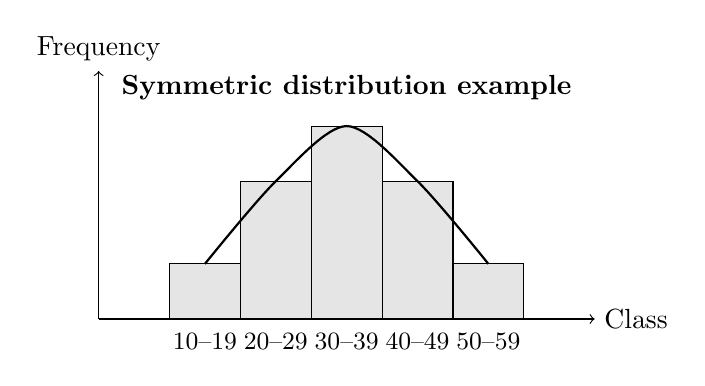
\begin{tikzpicture}[x=0.9cm,y=0.35cm]

% Axes
\draw[->] (0,0) -- (7,0) node[right]{Class};
\draw[->] (0,0) -- (0,9) node[above]{Frequency};

% Histogram bars (symmetric)
\draw[fill=gray!20] (1,0) rectangle (2,2);
\draw[fill=gray!20] (2,0) rectangle (3,5);
\draw[fill=gray!20] (3,0) rectangle (4,7);
\draw[fill=gray!20] (4,0) rectangle (5,5);
\draw[fill=gray!20] (5,0) rectangle (6,2);

% X-axis labels
\node at (1.5,-0.8) {\small 10--19};
\node at (2.5,-0.8) {\small 20--29};
\node at (3.5,-0.8) {\small 30--39};
\node at (4.5,-0.8) {\small 40--49};
\node at (5.5,-0.8) {\small 50--59};

% Trend line (smooth curve)
\draw[thick]
    plot[smooth] coordinates
    {(1.5,2) (2.5,5) (3.5,7) (4.5,5) (5.5,2)};

% Label
\node[align=center] at (3.5,8.4) {\textbf{Symmetric distribution example}};

\end{tikzpicture}
\end{center}




\section*{Chapter 2, Jan 9th}
\label{chap:two}


\underline{Experiment}: A process that generates an outcome.

\vspace{0.5em}

\underline{Sample Space ($S$)}: The set of all possible outcomes of an experiment.

\vspace{1em}

\textbf{Example 1:}

Select 3 items from a production line. Each item can be classified as either defective ($D$) or non-defective ($N$).

\[
S = \{ DDD, DDN, DND, NDD, DNN, NDN, NND, NNN \}
\]

Since each item has 2 possible outcomes,
\[
|S| = 2^3 = 8
\]

\vspace{1em}

\textbf{Example 2:}

\[
S = \{ (x,y) \mid x^2 + y^2 \le 4 \}
\]

\vspace{1em}

\underline{Event ($A$)}: A subset of the sample space $S$.

\vspace{0.5em}

\textbf{Examples of events:}
\[
A = \{ DDD, DDN, DND, NDD \}
\]
\[
B = \{ NNN \}
\]
\[
C = \{ (x,y) \mid x^2 + y^2 \le 4 \}
\]

\vspace{1em}

\underline{Event Operations}:
\begin{itemize}
  \item \underline{Complement}: $A^c$ (or $A'$)
  \item \underline{Intersection}: $A \cap B$
  \item \underline{Union}: $A \cup B$
  \item \underline{Null Event}: $\varnothing$
\end{itemize}

If
\[
A \cap B = \varnothing,
\]
then $A$ and $B$ are \underline{mutually exclusive}.

\vspace{1em}

\textbf{Example (Venn Diagram):}

\begin{center}
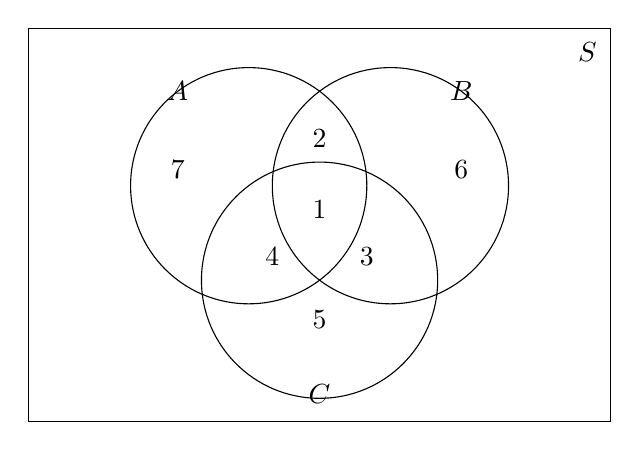
\begin{tikzpicture}[scale=1]

% Sample space
\draw (-2.8,-3) rectangle (4.6,2);

% Circles
\draw (0,0) circle (1.5);        % A
\draw (1.8,0) circle (1.5);      % B
\draw (0.9,-1.2) circle (1.5);   % C

% Labels
\node at (-0.9,1.2) {$A$};
\node at (2.7,1.2) {$B$};
\node at (0.9,-2.65) {$C$};
\node at (4.3,1.7) {$S$};

% Region numbers
\node at (-0.9,0.2) {7};        % A only
\node at (0.9,0.6) {2};         % A ∩ B
\node at (2.7,0.2) {6};         % B only
\node at (0.3,-0.9) {4};        % A ∩ C
\node at (1.5,-0.9) {3};        % B ∩ C
\node at (0.9,-0.3) {1};        % A ∩ B ∩ C
\node at (0.9,-1.7) {5};        % C only

\end{tikzpicture}
\end{center}

\[
A = \{ DDD, DDN, DND, NDD \}, \quad
B = \{ NNN \}
\]

\[
A \cup B = \{ DDD, DDN, DND, NDD, NNN \}
\]

\[
A \cap B = \varnothing
\]

\section*{Chapter 2: January 12}

\subsection*{Review}
{\itshape

\begin{enumerate}
    \item \underline{Experiment}: A process that generates an outcome.
    
    \item \underline{Sample Space} ($S$): The set of all possible outcomes of an experiment.
    
    \item \underline{Event Operations}:
    \begin{itemize}
        \item Complement: $A' \; (A^c)$
        \item Intersection: $A \cap B$
        \item Union: $A \cup B$
        \item Null Event: $\varnothing$
    \end{itemize}
    
    \item If $A \cap B = \varnothing$, then $A$ and $B$ are called \underline{mutually exclusive}.
\end{enumerate}

\fbox{
\parbox{0.95\textwidth}{
\[
(A \cap B)' = A' \cup B'
\]
\[
(A \cup B)' = A' \cap B'
\]
\[
A \cap \varnothing = \varnothing
\]
\[
A \cup \varnothing = A
\]
\[
A \cap (B \cup C) = (A \cap B) \cup (A \cap C)
\]
}}
}

\subsection*{Probability}

$P(A)$ = \underline{probability} of event $A$: the proportion of times the event occurs in infinitely many repetitions of the experiment.

\medskip

\textcolor{blue}{\textbf{Theorem2.1:}}
\[
0 \le P(A) \le 1
\]

\medskip

\fbox{
\parbox{0.95\textwidth}{
\[
P(A) + P(A') = 1
\]

\[
P(A \cup B) = P(A) + P(B) - P(A \cap B)
\]

\[
\begin{aligned}
P(A \cup B \cup C) =\;& P(A) + P(B) + P(C) \\
&- P(A \cap B) - P(A \cap C) - P(B \cap C) \\
&+ P(A \cap B \cap C)
\end{aligned}
\]
}}

\medskip

\subsection*{Mutually Exclusive Events}

\underline{Definition}:  
If $A_1, A_2, \ldots, A_n$ are mutually exclusive, then
\[
P(A_1 \cup A_2 \cup \cdots \cup A_n)
=
P(A_1) + P(A_2) + \cdots + P(A_n)
\]

If
\[
A_1 \cup A_2 \cup \cdots \cup A_n = S,
\]
then $\{A_1, A_2, \ldots, A_n\}$ is a \underline{partition} of $S$.

\medskip
\begin{figure}[H]
\centering
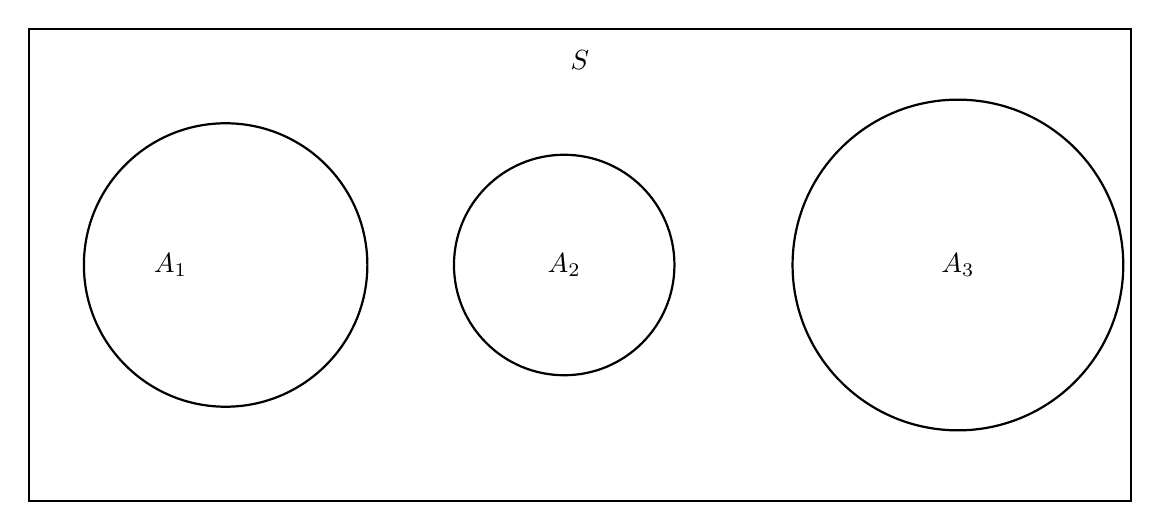
\begin{tikzpicture}[scale=1]

% Sample space
\draw[thick] (0,0) rectangle (14,6);
\node at (7,5.6) {$S$};

% A1
\draw[thick] (2.5,3) circle (1.8);
\node at (1.8,3) {$A_1$};

% A2
\draw[thick] (6.8,3) circle (1.4);
\node at (6.8,3) {$A_2$};

% A3
\draw[thick] (11.8,3) circle (2.1);
\node at (11.8,3) {$A_3$};

\end{tikzpicture}
\caption{Partition of the sample space $S$ into $A_1, A_2, A_3$}
\end{figure}


\subsection*{Example}

In a class of 33 students:
\begin{itemize}
    \item 17 earned an A on the midterm
    \item 14 earned an A on the final
    \item 11 earned no A on either exam
\end{itemize}

Find the probability that a randomly selected student earned A's on \underline{both} exams.

\begin{figure}[H]
\centering
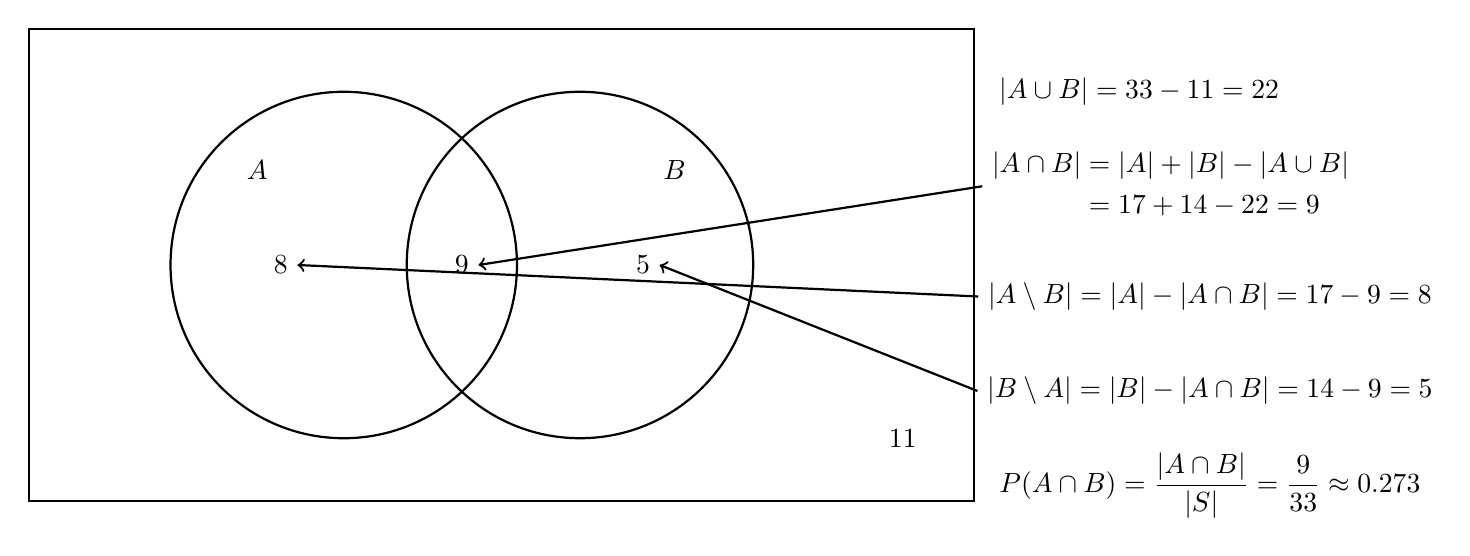
\begin{tikzpicture}[scale=1]

% -------------------------
% Sample space
% -------------------------
\draw[thick] (0,0) rectangle (12,6);

% -------------------------
% Circles A and B
% -------------------------
\draw[thick] (4,3) circle (2.2);
\draw[thick] (7,3) circle (2.2);

\node at (2.9,4.2) {$A$};
\node at (8.2,4.2) {$B$};

% -------------------------
% Region numbers
% -------------------------
\node (Aonly) at (3.2,3.0) {$8$};
\node (AB)    at (5.5,3.0) {$9$};
\node (Bonly) at (7.8,3.0) {$5$};
\node (outside) at (11.1,0.8) {$11$};

% -------------------------
% Calculation text blocks
% -------------------------
\node[align=left] (calcUnion) at (14.1 ,5.2) {$|A \cup B| = 33 - 11 = 22$};

\node[align=left] (calcInter) at (14.5,4.0) {$\begin{aligned}
|A \cap B|
&= |A| + |B| - |A \cup B| \\
&= 17 + 14 - 22 = 9
\end{aligned}$};

\node[align=left] (calcAonly) at (15,2.6) {$|A \setminus B| = |A| - |A \cap B| = 17 - 9 = 8$};

\node[align=left] (calcBonly) at (15,1.4) {$|B \setminus A| = |B| - |A \cap B| = 14 - 9 = 5$};

\node[align=left] (calcProb) at (15 ,0.2) {$P(A \cap B)=\dfrac{|A \cap B|}{|S|}=\dfrac{9}{33}\approx 0.273$};

% -------------------------
% Arrows pointing to regions
% -------------------------
\draw[->, thick] (calcInter.west) -- (AB.east);
\draw[->, thick] (calcAonly.west) -- (Aonly.east);
\draw[->, thick] (calcBonly.west) -- (Bonly.east);

\end{tikzpicture}
\caption{Events $A$: A on midterm, $B$: A on final, with region counts and calculations}
\end{figure}

\textcolor{blue}{\textbf{Theorem 2.2 (Equally Likely Outcomes):}}  

If the sample space $S$ has a finite number of outcomes and all outcomes are equally likely, then for any event $A$,
\[
P(A) = \frac{|A|}{|S|}
\]

where  \\
\text{A: the event of interest (a subset of the sample space $S$),}\\
\text{S: the sample space, i.e.\ the set of all possible outcomes.}


\subsection*{Example 1: Poker Hands Basics}

A standard deck has:
\[
4 \text{ suits} \times 13 \text{ denominations (A,2,3,\ldots,Q,K)} = 52 \text{ cards}.
\]

A poker hand consists of 5 cards chosen from 52:
\[
|S| = \binom{52}{5} = 2,\!598,\!960.
\]

\subsection*{Combinations Reminder}

If there are 3 objects $\{A,B,C\}$ and we choose 2:
\[
\binom{3}{2} = \frac{3!}{(3-2)!2!}.
\]

Order does \underline{not} matter.

\subsection*{Example 2: Probability of 2 Aces and 1 Jack}

A 5-card hand contains:
\begin{itemize}
    \item exactly 2 aces,
    \item exactly 1 jack,
    \item 2 cards that are neither aces nor jacks.
\end{itemize}


\[
P(\text{2 aces and 1 jack})
=
\frac{\binom{4}{2}\binom{4}{1}\binom{44}{2}}{\binom{52}{5}}.
\]

\subsection*{Example 3: Probability of a Full House}

A full house consists of:
\begin{itemize}
    \item 3 cards of one denomination
    \item 2 cards of a different denomination
\end{itemize}

Number of full house hands:
\[
\binom{13}{1} \binom{4}{3}
\binom{12}{1} \binom{4}{2}.
\]

Thus,
\[
P(\text{full house})
=
\frac{\binom{13}{1}\binom{4}{3}\binom{12}{1}\binom{4}{2}}{\binom{52}{5}}.
\]

\subsection*{Example 4: Probability of Four of a Kind}

A four of a kind consists of:
\begin{itemize}
    \item 4 cards of the same denomination
    \item 1 remaining card of a different denomination
\end{itemize}

Number of such hands:
\[
\binom{13}{1}\binom{4}{4}\binom{48}{1}.
\]

Thus,
\[
P(\text{four of a kind})
=
\frac{\binom{13}{1}\binom{4}{4}\binom{48}{1}}{\binom{52}{5}}.
\]


\subsection*{Example 5: Probability of Exactly One Pair}

An \textbf{excatly} one-pair hand consists of:
\begin{itemize}
    \item 1 pair
    \item 3 cards of different denominations, none matching the pair
\end{itemize}

Number of such hands:
\[
\binom{13}{1}\binom{4}{2}
\binom{12}{3}\binom{4}{1}^3.
\]

Thus,
\[
P(\text{exactly one pair})
=
\frac{
\binom{13}{1}\binom{4}{2}
\binom{12}{3}\binom{4}{1}^3
}{
\binom{52}{5}
}.
\]

\subsection*{Note*: Counting Patterns }

\[
\binom{a}{b}
\]

\textbf{Meaning:} Choose b different items from $a$ \textbf{at once}, order does not matter.

\textbf{Key features:}
\begin{itemize}
    \item No repeats
    \item Grouped choice
    \item Used when items must be \underline{distinct}
\end{itemize}

\vspace{0.5em}

\[
\binom{a}{1}^b
\]

\textbf{Meaning:} Make $b$ \underline{independent choices}, each time choosing 1 item from $c$.

\textbf{Key features:}
\begin{itemize}
    \item Repeats allowed
    \item Choices are independent
    \item Used when selections do \underline{not} restrict each other
\end{itemize}

\vspace{0.5em}

\noindent
\textcolor{red}{\textbf{Rule to Remember:}}

\[
\textcolor{red}{\text{Different items, no repeats } \Rightarrow \binom{a}{b}}
\]

\[
\textcolor{red}{\text{Independent choices } \Rightarrow \binom{c}{1}^b}
\]

\section*{Chapter 2 continue, Jan 14}

\subsection*{Review}

\begin{enumerate}
    \item \textit{\underline{Probability} is the proportion of times the event occurs in infinitely many repetitions of
the experiment.}

    \item \textit{$0 \le P(A) \le 1$}

    \item \textit{$P(A) + P(A^c) = 1$}

    \item \textit{$P(A \cup B) = P(A) + P(B) - P(A \cap B)$}

    \item \textit{
    $
    \begin{aligned}
    P(A \cup B \cup C)
    &= P(A) + P(B) + P(C) \\
    &\quad - P(A \cap B) - P(A \cap C) - P(B \cap C) \\
    &\quad + P(A \cap B \cap C)
    \end{aligned}
    $
    }

    \item \textit{\underline{Permutation}: A permutation counts ordered arrangements.}

    \[
    \boxed{
    {}_nP_r = \frac{n!}{(n-r)!}
    }
    \]
\end{enumerate}


\subsection*{Example 1: Two fair dice}

A pair of fair dice are rolled. Find the probability that the second die lands on a smaller value than the first.

The outcomes where the second die is smaller than the first are represented below.

\[
\begin{array}{c|l}
\text{First Die (Stem)} & \text{Second Die (Leaf)} \\ \hline
2 & 1 \\
3 & 1\;2 \\
4 & 1\;2\;3 \\
5 & 1\;2\;3\;4 \\
6 & 1\;2\;3\;4\;5
\end{array}
\]

There are 15 favorable outcomes and 36 total outcomes.

\[
P(\text{second}<\text{first}) = \frac{15}{36} = \frac{5}{12}.
\]

\subsection*{\underline{Conditional Probability}}

The conditional probability of an event $B$ given that event $A$ has occurred is the probability that $B$ occurs when it is known that $A$ has occurred.

\[
\boxed{
P(B \mid A) = \frac{P(A \cap B)}{P(A)}, \quad P(A) > 0
}
\]

\subsection*{Example 2: Drinking Survey}

\textit{
A survey records the following data:
}

\[
\begin{array}{c|cc|c}
 & D & N & \text{Total} \\ \hline
M & 19 & 41 & 60 \\
F & 12 & 28 & 40 \\ \hline
\text{Total} & 31 & 69 & 100
\end{array}
\]
The symbols used above are defined as follows:

\begin{itemize}
    \item $M$: male
    \item $F$: female
    \item $D$: the individual drinks
    \item $N$: the individual does not drink
\end{itemize}

\[
P(D|M) = \frac{19}{60}
\qquad
P(M|D) = \frac{19}{31}
\]

\subsection*{Law of Total Probability}

\textcolor{blue}{
Theorem 2.3: If $B_1, \ldots, B_k$ form a partition (do not overlap but covers the whole sample space) of $S$ with $P(B_i)>0$, then for any event $A$,
}

\[
P(A) = \sum_{i=1}^k P(A|B_i)P(B_i)
\]
\subsection*{Example 3: Monty Hall (3 doors)}

\begin{center}
\renewcommand{\arraystretch}{1.25}
\begin{tabular}{c|c|c|c|c}
Car location & Monty opens & Probability & Stay & Switch \\ \hline
Door 1 & Door 2 & $\frac{1}{6}$ & Car & Goat \\ \hline
Door 1 & Door 3 & $\frac{1}{6}$ & Car & Goat \\ \hline
Door 2 & Door 3 & $\frac{1}{3}$ & Goat & Car \\ \hline
Door 3 & Door 2 & $\frac{1}{3}$ & Goat & Car
\end{tabular}
\end{center}

Staying wins only when the car is behind Door 1, so
\[
P(\text{win by staying})=\frac{1}{6}+\frac{1}{6}=\frac{1}{3}.
\]

Switching wins when the car is behind Door 2 or Door 3, so
\[
P(\text{win by switching})=\frac{1}{3}+\frac{1}{3}=\frac{2}{3}.
\]

\subsection*{Example 4: Birthday Problem}

Assume the following:
\begin{itemize}
    \item Leap years are ignored
    \item All 365 birthdays are equally likely
    \item Birthdays of different people are independent
\end{itemize}

\textbf{Question:}  
What is the probability that at least two people share the same birthday in a group of $n$ people?

\medskip

Rather than computing this directly, we use the complement rule.

\[
P(\text{at least one match}) = 1 - P(\text{no match})
\]

\subsubsection*{Probability of no shared birthdays}

\begin{itemize}
    \item Person 1 can have any birthday: probability $1$
    \item Person 2 must avoid that birthday: $\frac{364}{365}$
    \item Person 3 must avoid the first two birthdays: $\frac{363}{365}$
    \item $\dots$
    \item Person $n$ must avoid the previous $n-1$ birthdays: $\frac{365-(n-1)}{365}$
\end{itemize}

Therefore,

\[
P(\text{no match})
=
\frac{365}{365}
\cdot
\frac{364}{365}
\cdot
\frac{363}{365}
\cdots
\frac{365-(n-1)}{365}
\]

or equivalently,

\[
P(\text{no match})
=
\prod_{k=0}^{n-1} \frac{365-k}{365}
\]

\subsubsection*{Final result}

\[
P(\text{at least one shared birthday})
=
1
-
\prod_{k=0}^{n-1} \frac{365-k}{365}
\]

\subsubsection*{Important values}

\begin{itemize}
    \item For $n = 23$: \quad $P(\text{at least one match}) \approx 0.507$
    \item For $n = 57$: \quad $P(\text{at least one match}) \approx 0.99$
\end{itemize}

\section*{Chapter 2 — Jan 16}

\begin{itshape}

\subsection*{Review: Conditional Probability}

\underline{Conditional Probability:}

The probability of event $B$ given that event $A$ has occurred is

\[
\boxed{
P(B \mid A) = \frac{P(A \cap B)}{P(A)}, \quad P(A) > 0
}
\]

Read as: the probability of $B$ given $A$.

\end{itshape}



\subsection*{Independence of Events}

Definition (Independence): Events $A$ and $B$ are \underline{independent} if and only if

\[
\boxed{
P(B \mid A) = P(B)
}
\]

Equivalently,

\[
P(A \mid B) = P(A)
\]

or

\[
\boxed{
P(A \cap B) = P(A)\,P(B)
}
\]

\subsection*{Multiple Independent Events}

\underline{Definition:}

If events $A_1, A_2, \ldots, A_k$ are independent, then

\[
\boxed{
P(A_1 \cap A_2 \cap \cdots \cap A_k)
= P(A_1)\,P(A_2)\cdots P(A_k)
}
\]


\subsection*{Mutual Independence}

\underline {Mutual Independence} : A collection of events $A_1, A_2, \ldots, A_n$ is \underline{mutually independent} if and only if
for \textit{every} subcollection $\{A_{i_1}, \ldots, A_{i_k}\}$,


\[
\boxed{
P\!\left(\bigcap_{j=1}^{k} A_{i_j}\right)
= \prod_{j=1}^{k} P(A_{i_j})
}
\]

Example (Three Events):

Events $A_1, A_2, A_3$ are mutually independent if all of the following hold:

\[
P(A_1 \cap A_2) = P(A_1)P(A_2)
\]

\[
P(A_1 \cap A_3) = P(A_1)P(A_3)
\]

\[
P(A_2 \cap A_3) = P(A_2)P(A_3)
\]

\[
P(A_1 \cap A_2 \cap A_3)
= P(A_1)P(A_2)P(A_3)
\]
\textit{
\underline{Note:} Mutually exclusive events are \underline{dependent}.
If one event occurs, the other cannot occur.
}


\subsection*{Example: Component Reliability }

An electrical system has four components $A,B,C,D$.
The system works if $A$ and $B$ work and at least one of $C$ or $D$ works.
Assume all components are independent.
\begin{center}
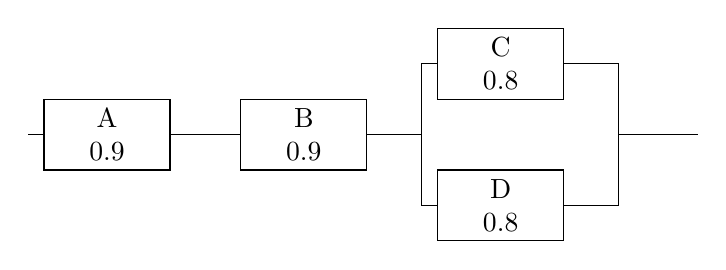
\begin{tikzpicture}[
    scale=1,
    every node/.style={
        draw,
        rectangle,
        minimum width=1.6cm,
        minimum height=0.9cm,
        align=center
    }
]

% Nodes
\node (A) at (0,0) {A \\ 0.9};
\node (B) at (2.5,0) {B \\ 0.9};

\node (C) at (5,0.9) {C \\ 0.8};
\node (D) at (5,-0.9) {D \\ 0.8};

% Connections
\draw (-1,0) -- (A);
\draw (A) -- (B);
\draw (B) -- (4,0);

\draw (4,0) -- (4,0.9) -- (C);
\draw (4,0) -- (4,-0.9) -- (D);

\draw (C) -- (6.5,0.9) -- (6.5,0);
\draw (D) -- (6.5,-0.9) -- (6.5,0);

\draw (6.5,0) -- (7.5,0);

\end{tikzpicture}
\end{center}

\[
P(A)=0.9,\quad P(B)=0.9,\quad P(C)=0.8,\quad P(D)=0.8
\]
\subsubsection*{(a) Probability the entire system works}

The system works if $A$ and $B$ work and either $C$ or $D$ works.

\[
\begin{aligned}
P(\text{system works})
&= P(\text{all work}) 
+ P(A,B,C \text{ work}, D \text{ does not}) \\
&\quad + P(A,B,D \text{ work}, C \text{ does not})
\end{aligned}
\]

\[
= (0.9)(0.9)(0.8)(0.8)
+ (0.9)(0.9)(0.8)(1-0.8)
+ (0.9)(0.9)(0.8)(1-0.8)
\]

\[
\boxed{
P(\text{system works}) = 0.7776
}
\]

\subsubsection*{(b) Conditional probability}

\[
P(C^c \mid \text{system works})
= \frac{P(C^c \cap \text{system works})}{P(\text{system works})}
\]

\[
P(C^c \cap \text{system works})
= (0.9)(0.9)(0.8)(1-0.8)
\]

\[
\boxed{
P(C^c \mid \text{system works})
= \frac{(0.9)(0.9)(0.8)(1-0.8)}{0.7776}
= 0.16
}
\]

\subsection*{\textcolor{blue}{Theorem of Total Probability}}

Let $B_1, B_2, \ldots, B_k$ be a partition of the sample space $S$ with
$P(B_i) > 0$ for all $i$.
Then for any event $A \subseteq S$,

\[
\boxed{
P(A)
= \sum_{i=1}^{k} P(A \mid B_i)\,P(B_i)
= \sum_{i=1}^{k} P(A \cap B_i)
}
\]

\subsection*{\textcolor{blue}{Theorem: Bayes' Rule (1701--1761)}}

Let $B_1, B_2, \ldots, B_k$ be a partition of the sample space $S$ such that
$P(B_i) > 0$ for $i = 1,\ldots,k$.
For any event $A \subseteq S$ (in) with $P(A) > 0$,
\
\[
\boxed{
P(B_r \mid A)
= \frac{P(B_r \cap A)}{\sum_{i=1}^{k} P(B_i \cap A)}
= \frac{P(B_r)\,P(A \mid B_r)}{\sum_{i=1}^{k} P(B_i)\,P(A \mid B_i)},
\quad r = 1,\ldots,k
}
\]

\begin{figure}[h]
\centering
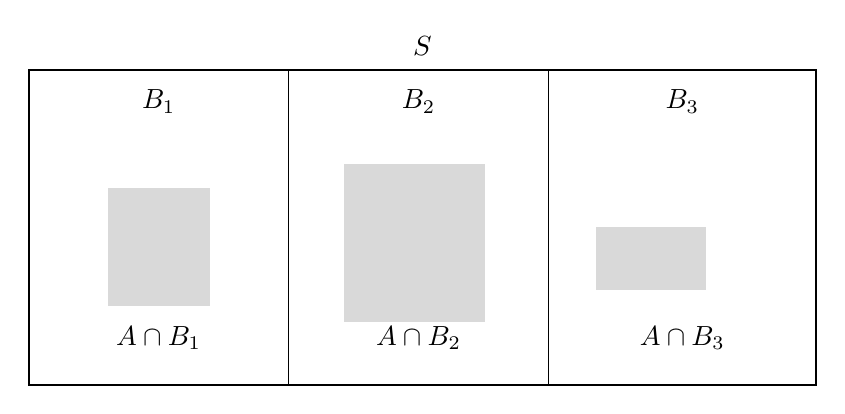
\begin{tikzpicture}[scale=1]

% Sample space
\draw[thick] (0,0) rectangle (10,4);
\node at (5,4.3) {$S$};

% Partition blocks
\draw (0,0) rectangle (3.3,4);
\draw (3.3,0) rectangle (6.6,4);
\draw (6.6,0) rectangle (10,4);

\node at (1.65,3.6) {$B_1$};
\node at (4.95,3.6) {$B_2$};
\node at (8.3,3.6) {$B_3$};

% Event A intersections
\fill[gray!30] (1,1) rectangle (2.3,2.5);
\fill[gray!30] (4,0.8) rectangle (5.8,2.8);
\fill[gray!30] (7.2,1.2) rectangle (8.6,2);

\node at (1.65,0.6) {$A\cap B_1$};
\node at (4.95,0.6) {$A\cap B_2$};
\node at (8.3,0.6) {$A\cap B_3$};

\end{tikzpicture}
\caption{Visual interpretation of Bayes’ Rule}
\end{figure}


\subsection*{Example (Medical Test)}

The fraction of people in a population who have a certain disease is $0.01$.

\[
P(D) = 0.01, \quad P(D^c) = 0.99
\]

The test characteristics are:
\[
P(\text{test says } D \mid D^c) = 0.05
\quad \text{(false positive rate)}
\]

\[
P(\text{test says } D^c \mid D) = 0.20
\quad \text{(false negative rate)}
\]

Thus,
\[
P(\text{test says } D \mid D) = 1 - 0.20 = 0.80
\]

\textit{
\underline{Note:}
$1 - P(\text{test says } D^c \mid D)$ is called the \underline{sensitivity} of the test,
and $1 - P(\text{test says } D \mid D^c)$ is called the \underline{specificity}.
}


\subsubsection*{(a) Probability the test says disease}

\[
P(\text{test says } D)
= P(D \cap \text{test says } D)
+ P(D^c \cap \text{test says } D)
\]

\[
= P(\text{test says } D \mid D)P(D)
+ P(\text{test says } D \mid D^c)P(D^c)
\]

\[
= (0.80)(0.01) + (0.05)(0.99)
= 0.0575
\]


\subsubsection*{(b) Probability of disease given positive test}

\[
P(D \mid \text{test says } D)
= \frac{P(D \cap \text{test says } D)}{P(\text{test says } D)}
\]

\[
= \frac{P(\text{test says } D \mid D)P(D)}{0.0575}
= \frac{(0.80)(0.01)}{0.0575}
\]

\[
\boxed{
P(D \mid \text{test says } D) \approx 0.139
}
\]


\subsubsection*{(c) Probability of disease given negative test}

\[
P(D \mid \text{test says } D^c)
= \frac{P(D \cap \text{test says } D^c)}{P(\text{test says } D^c)}
\]

\[
= \frac{P(\text{test says } D^c \mid D)P(D)}{1 - P(\text{test says } D)}
\]

\[
= \frac{(0.20)(0.01)}{1 - 0.0575}
\]

\[
\boxed{
P(D \mid \text{test says } D^c) \approx 0.00212
}
\]

\end{document}
